\section{Experiments}
\begin{table*}[t]
\begin{center}
 \caption{The performance comparison between PRP and other methods. The best results are boldfaced, and the improvements are significant over the BPR under a two-sided t-test with $p<0.05$.}
\label{tab:Overall-comprehension}
\begin{tabular}{@{}llccccccc@{}}
\toprule
\textbf{Dataset} & \textbf{Methods} & HR@10 & HR@20 & Recall@10 & Recall@20 & NDCG@10 & NDCG@20  \\ \midrule
\multirow{8}{*}{ML-1M} 
  & \textbf{BPR} & 0.7419 & 0.8374 & 0.1635 & 0.2502 & 0.2554 &  0.2619 \\
  & \textbf{SRNS} & 0.7611 & 0.8533 & 0.1746 & 0.2618 & 0.2639 &  0.2687 \\
 & \textbf{MixGCF} & 0.7601 & 0.8483 & 0.1739 & 0.2604 & 0.2657 & 0.2702  \\
 & \textbf{UIB} & 0.7346 & 0.8318 & 0.1559 & 0.2406 & 0.2453 & 0.2520 \\ 
& \textbf{SimpleX} & 0.7586 & 0.8518 & 0.1709 & 0.2573 & 0.2626 & 0.2675  \\ 
& \textbf{ANS} & 0.7675 & 0.8583 & 0.1759 & 0.2625 & 0.2624 & 0.2683  \\
& \textbf{PRP} & \textbf{0.7796}& \textbf{0.8657} & \textbf{0.1866} & \textbf{0.2765} & \textbf{0.2822 }& \textbf{0.2874} \\ 
\cmidrule{2-8}
& \textbf{Improvement} & \textbf{5.08\%}& \textbf{3.38\%} & \textbf{14.13\%} & \textbf{10.51\%} & \textbf{10.49\%}& \textbf{9.74\%} \\ 

 \midrule
 
\multirow{8}{*}{Gowalla} 
  & \textbf{BPR} & 0.1989 & 0.2763 & 0.0938 & 0.1389 & 0.0674 &  0.0804 \\
  & \textbf{SRNS} & 0.2295 & 0.3177 & 0.1171 & 0.1711 & 0.0814 & 0.0972  \\ 
 & \textbf{MixGCF} & 0.2401 & 0.3254 & 0.1189 & 0.1728 & 0.0853 & 0.1008  \\
 & \textbf{UIB} & 0.2275 & 0.3161 & 0.1140 & 0.1695 & 0.0794 & 0.0954 \\ 
& \textbf{SimpleX} & 0.2192 & 0.3082 & 0.1074 & 0.1617 & 0.0736 & 0.0892  \\
& \textbf{ANS} & 0.2467 & 0.3317 & 0.1206 & 0.1756 & 0.0869 & 0.1027  \\ 
& \textbf{PRP} & \textbf{0.2528} & \textbf{0.3395} & \textbf{0.1229} & \textbf{0.1777} & \textbf{0.0884} &\textbf{0.1040}  \\ 
\cmidrule{2-8}
& \textbf{Improvement} & \textbf{27.10\%}& \textbf{22.87\%} & \textbf{31.02\%} & \textbf{27.93\%} & \textbf{31.16\% }& \textbf{29.35\%} \\ 

 \midrule

 \multirow{8}{*}{Foursquare} 
   & \textbf{BPR} & 0.1717 & 0.2336 & 0.0262 & 0.0381 & 0.0283 &  0.0328 \\
  & \textbf{SRNS} & 0.1948 & 0.2596 & 0.0314 & 0.0418 & 0.0351 & 0.0392\\
 & \textbf{MixGCF} & 0.1994 & 0.2752 & 0.0316 & 0.0458 & 0.0351 & 0.0405  \\
 & \textbf{UIB} & 0.1662 & 0.2299 & 0.0265 & 0.0375 & 0.0280 & 0.0322 \\ 
& \textbf{SimpleX} & 0.1801 & 0.2650 & 0.0267 & 0.0421 & 0.0267 & 0.0329  \\ 
& \textbf{ANS} & 0.1958 & \textbf{0.2798} & 0.0303 & 0.0461 & 0.0321 & 0.0386  \\ 
& \textbf{PRP} & \textbf{0.2124} & 0.2752 & \textbf{0.0332} & \textbf{0.0461} & \textbf{0.0367} & \textbf{0.0413} \\ 
\cmidrule{2-8}
& \textbf{Improvement} & \textbf{23.70\%}& \textbf{17.81\%} & \textbf{26.72\%} & \textbf{20.73\%} & \textbf{29.68\%}& \textbf{25.91\%} \\ 
 
 \midrule
 
\multirow{8}{*}{Yelp} 
   & \textbf{BPR} & 0.1537 & 0.2398 & 0.0427 & 0.0717 & 0.0334 &  0.0432 \\
  & \textbf{SRNS} & 0.1834 & 0.2779 & 0.0520 & 0.0862 & 0.0406 & 0.0522 \\
 % \cmidrule(l){2-9} 
 & \textbf{MixGCF} & 0.1891 & 0.2781 & 0.0538 & 0.0871 & 0.0424 & 0.0536  \\
 & \textbf{UIB} & 0.1592 & 0.2504 & 0.0445 & 0.0756 & 0.0350  & 0.0455 \\ 
& \textbf{SimpleX} & 0.1850 & 0.2780 & 0.0519 & 0.0861 & 0.0410 & 0.0524  \\ 
& \textbf{ANS} & 0.1844 & 0.2777 & 0.0524 & 0.0862 & 0.0414 & 0.0527  \\ 
& \textbf{PRP} & \textbf{0.2000} & \textbf{0.2940} & \textbf{0.0577} & \textbf{0.0928} & \textbf{0.0464} & \textbf{0.0581} \\ 
\cmidrule{2-8}
& \textbf{Improvement} & \textbf{30.12\%}& \textbf{22.60\%} & \textbf{35.13\%} & \textbf{29.43\%} & \textbf{38.92\%}& \textbf{34.49\%} \\ 

 \bottomrule
 \end{tabular}
  \end{center}
\end{table*}
In this section, we conduct comprehensive experiments to demonstrate the performance of PRP.
\subsection{Experimental Settings}
\textbf{Datasets}. We evaluate PRP on four widely used public real-world datasets: (1) \textbf{MovieLens} contains user ratings on movies. We use 1M versions and treat rating movies as interacted items. (2) \textbf{Yelp} contains user reviews of restaurants and bars after Jan.1st, 2018. (3) \textbf{Gowalla} is a check-in dataset where users share their locations. (4) \textbf{Foursquare} consists of check-ins in NYC and Tokyo over approximately 10 months. These datasets have different statistical properties, which can reliably validate the performance of a model~\cite{CCC22}.

\textbf{Baselines}. 
To assess the effectiveness of PRP, we compare it against several competitive methods that represent different research directions: \textbf{BPR}~\cite{RFG12}, \textbf{SimpleX}~\cite{MZW21},  \textbf{UIB}~\cite{ZZY22}, \textbf{SRNS}~\cite{DQY20},\textbf{MixGCF}~\cite{HDD21}, \textbf{ANS}~\cite{ZCL23}. 
Furthermore, to validate the broad applicability of PRP, we integrate it with various mainstream CF models, including: \textbf{MF}~\cite{RFG12}, \textbf{NGCF}~\cite{WHW19}, and \textbf{LightGCN}~\cite{HDW20}.


All data preprocessing, dataset partitioning and implementation of the methods are carried out using the RecBole v1.1.1 framework~\cite{ZMH21}. 


\subsection{Overall Performance}
\begin{table*}[t]
\caption{Experimental results of different CF models with (w) or without (w/o) the PRP.}
\centering
\begin{tabular}{@{}llcccccccc@{}}
\toprule
\multirow{2}{*}{\textbf{Dataset}} & \multirow{2}{*}{\textbf{Metric}} & \multicolumn{2}{c}{\textbf{MF}} & \multicolumn{2}{c}{\textbf{LightGCN}} & \multicolumn{2}{c}{\textbf{NGCF}} & 
\\ \cmidrule(l){3-9} 
 &  & w/o & w & w/o & w & w/o & w  \\ \midrule
\multirow{6}{*}{Yelp} 
 & Recall@10 & 0.0427 & \textbf{0.0577} & 0.0543 & \textbf{0.0655} & 0.0439 & \textbf{0.0514}  \\
 & Recall@20 & 0.0717 & \textbf{0.0928} & 0.0884 & \textbf{0.1044} & 0.0738 & \textbf{0.0834}   \\
 & HR@10 & 0.1537 & \textbf{0.2000} & 0.1896 & \textbf{0.2210} & 0.1593 & \textbf{0.1811}   \\
 & HR@20 & 0.2398 & \textbf{0.2940} & 0.2847 & \textbf{0.3232} & 0.2460 & \textbf{0.2705}  \\
 & NDCG@10 & 0.0334 & \textbf{0.0464} & 0.0432 & \textbf{0.0525} & 0.0345 & \textbf{0.0406}  \\
 & NDCG@20 & 0.0432 & \textbf{0.0581} & 0.0546 & \textbf{0.0655} & 0.0447 & \textbf{0.0512}   \\
\cmidrule(l){2-9} 
  & Improvement &  & \textbf{31.78\%} &  & \textbf{18.38\%} &  & \textbf{14.33\%} \\ \midrule 

\multirow{6}{*}{Gowalla} 
 & Recall@10 & 0.0938 & \textbf{0.1236} & 0.1280 & \textbf{0.1360} & 0.1011 & \textbf{0.1225}   \\
 & Recall@20 & 0.1389 & \textbf{0.1787} & 0.1849 & \textbf{0.1967} & 0.1490 & \textbf{0.1745}   \\
 & HR@10 & 0.1989 & \textbf{0.2534} &  0.2553 & \textbf{0.2712} & 0.2110 & \textbf{0.2468}  \\
 & HR@20 & 0.2763 & \textbf{0.3366} & 0.3432 & \textbf{0.3626} & 0.2900 & \textbf{0.3321}   \\
 & NDCG@10 & 0.0674 & \textbf{0.0896} & 0.0917 & \textbf{0.0981} & 0.0722 & \textbf{0.0856} \\
 & NDCG@20 & 0.0804 & \textbf{0.1052} & 0.1079 & \textbf{0.1155} & 0.0859 &  \textbf{0.1010}  \\
\cmidrule(l){2-9} 
  & Improvement &  & \textbf{29.91\%} &  & \textbf{6.42\%} &  & \textbf{17.65\%} \\ \midrule 
\end{tabular}
\label{tab:with}
\end{table*}
Table~\ref{tab:Overall-comprehension} presents the performance results of PRP compared to several baseline methods. We also integrated PRP with various mainstream CF models, as shown in Table~\ref{tab:with}. The reported improvements are statistically significant under a two-sided t-test with $p < 0.05$. Our observations are as follows: 
(1) PRP consistently achieves state-of-the-art results across almost all cases. Notably, it significantly outperforms traditional methods like BPR, with the highest improvement of 38.9\% observed on the Yelp dataset. This underscores the substantial performance gains achieved by incorporating ranking information into the model.
(2) Negative sampling (NS) methods achieve sub-optimal results. While NS methods can capture information from sub-rankings where $k>2$, BPR is limited to $k=2$. This ability of NS methods to utilize more extensive sub-ranking information explains their improved performance over BPR. However, NS methods still overlook other sub-ranking information, leading to their lower performance compared to PRP.
(3)  Methods such as ANS and MixGCF generate harder synthetic negative samples $i_n^{syn}$, leading to impressive results. This is reasonable, as generating harder $i_n^{syn}$ implicitly aligns with the ranking information $i_n^{syn} > i_n$. However, synthesizing these negative samples requires careful design and involves significant computational overhead. Moreover, since only a specific ranking is considered, there remains a performance gap when compared to PRP. (4) Methods such as SimpleX use large numbers of negative samples to construct more pairwise interactions. Although they have the potential to recover ranking information if we have $\Omega(|U|N^2)$ accurate pairs~\cite{ABB94,MG17}, this is impractical in real-world scenarios~\cite{LSC21,LGZ24}. (5) As shown in Table~\ref{tab:with}, integrating PRP leads to significant performance improvements for all base models in all cases. Surprisingly, even with a simple BPR-MF model, PRP achieves performance comparable to more sophisticated GNN models. This demonstrates the superior effectiveness and broad applicability of the PRP approach.

\subsection{In-depth Analysis}
\begin{figure*}[t]
\center
\subfigure[Foursquare]{
\begin{minipage}[t]{0.235\linewidth} 
\centering
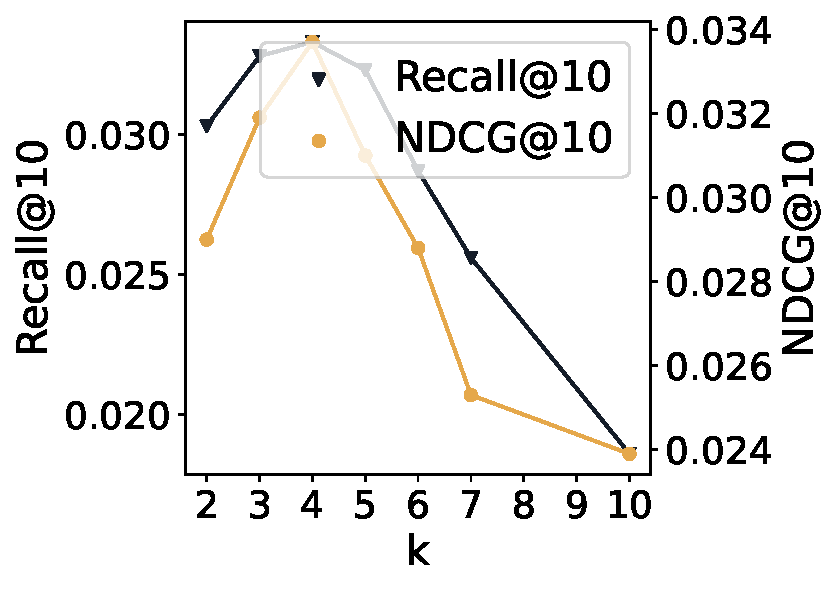
\includegraphics[width=\linewidth]{fig/k_four.pdf}
\label{fig:k_four}
\end{minipage}
}
\subfigure[Gowalla]{
\begin{minipage}[t]{0.227\linewidth}
\centering
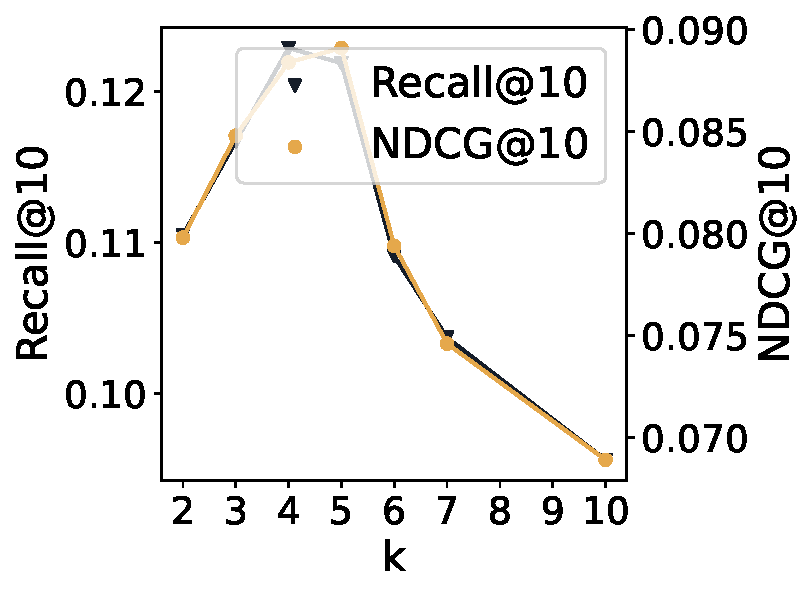
\includegraphics[width=\linewidth]{fig/k_Gowalla.pdf}
\label{fig:k_Gowalla}

\end{minipage}
}
\subfigure[Foursquare]{
\begin{minipage}[t]{0.232\linewidth}
\centering
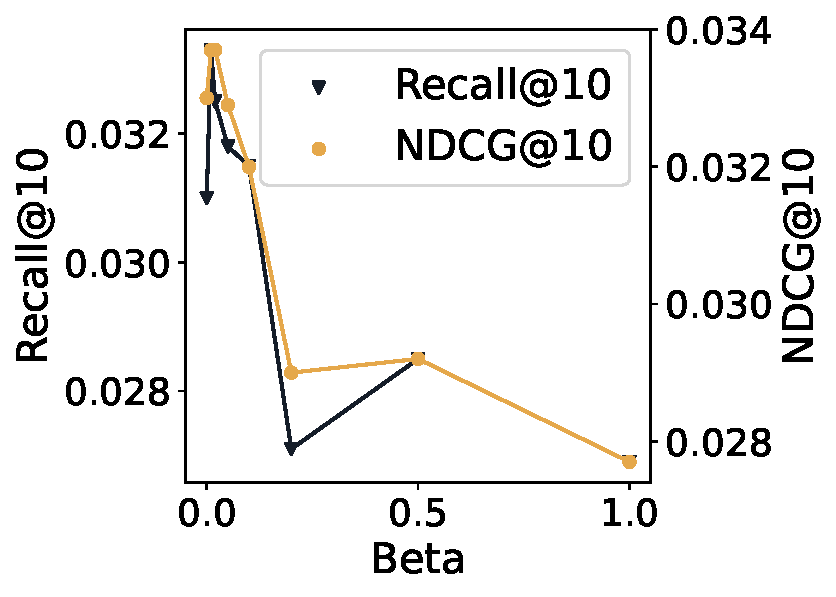
\includegraphics[width=\linewidth]{fig/beta_four.pdf}
\label{fig:beta_four}
\end{minipage}
}
\subfigure[Gowalla]{
\begin{minipage}[t]{0.238\linewidth}
\centering
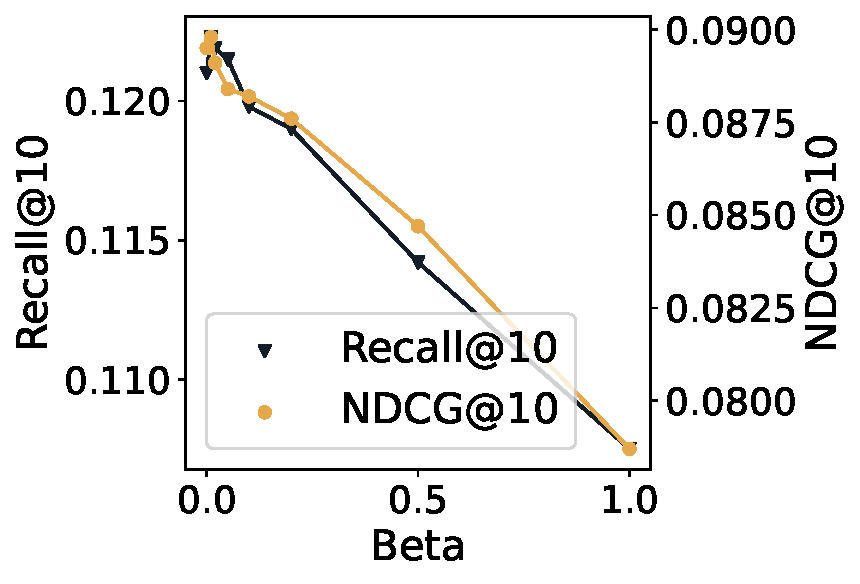
\includegraphics[width=\linewidth]{fig/beta_Gowalla.pdf}
\label{fig:beta_Gowalla}
\end{minipage}
}
\caption{Experiments to demonstrate the influence of ranking length and supervised magnitude.}
\vspace{-4mm}
\end{figure*}

\textbf{Ranking Length}. The parameter $k$ determines the number of items to be ranked. Intuitively, the larger the $k$, the closer it approximates the full ranking needed for ideal CF, potentially enhancing performance. However, as $k$ increases, ranking becomes more challenging. Due to data quality limitations, model capacity, and inherent noise, it is impractical to let $k$ increase indefinitely. Experimental results presented in Figure~\ref{fig:k_four}, ~\ref{fig:k_Gowalla} confirm this, showing a sharp performance drop for $k>5$, indicating the ranker's inability to accurately rank and the detrimental impact of incorrect rankings on model performance. Additionally, a larger $k$ affects the method's efficiency, necessitating careful selection based on the specific application scenario.

\textbf{Supervised Magnitude}. The parameter $\beta$ adjusts the supervised magnitude of $L_p$ on the ranker. Experimental results, presented in Figure~\ref{fig:beta_four}, ~\ref{fig:beta_Gowalla}, show that performance initially increases with $\beta$ but decreases beyond a certain point. Initially, a higher $\beta$ allows $L_p$ to provide more information for ranker training, improving pseudo-ranking quality. However, an excessively high $\beta$ simplifies the noise injection ranking problem too much, making $L_p$ optimization easier than the recommendation task. This shifts the model's focus away from the recommendation task, degrading performance.
\begin{figure*}[t]
\center
\subfigure[Foursquare]{
\begin{minipage}[t]{0.256\linewidth} 
\centering
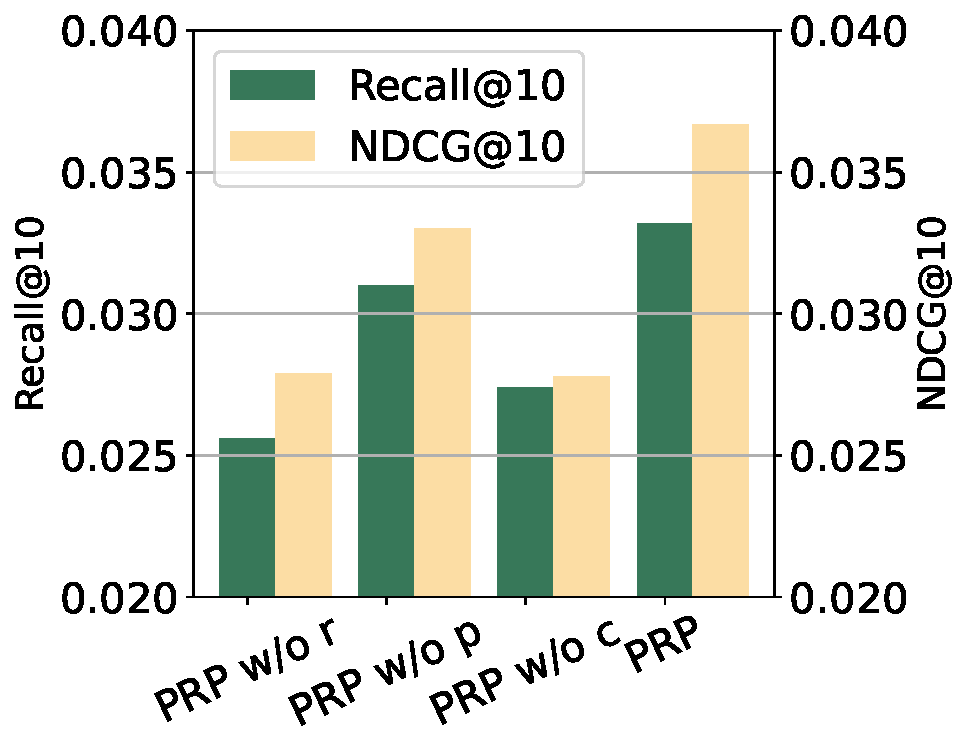
\includegraphics[width=\linewidth]{fig/ablation_foursquare.pdf}
\label{fig:ablation_foursquare}
\end{minipage}
}
\subfigure[Gowalla]{
\begin{minipage}[t]{0.242\linewidth}
\centering
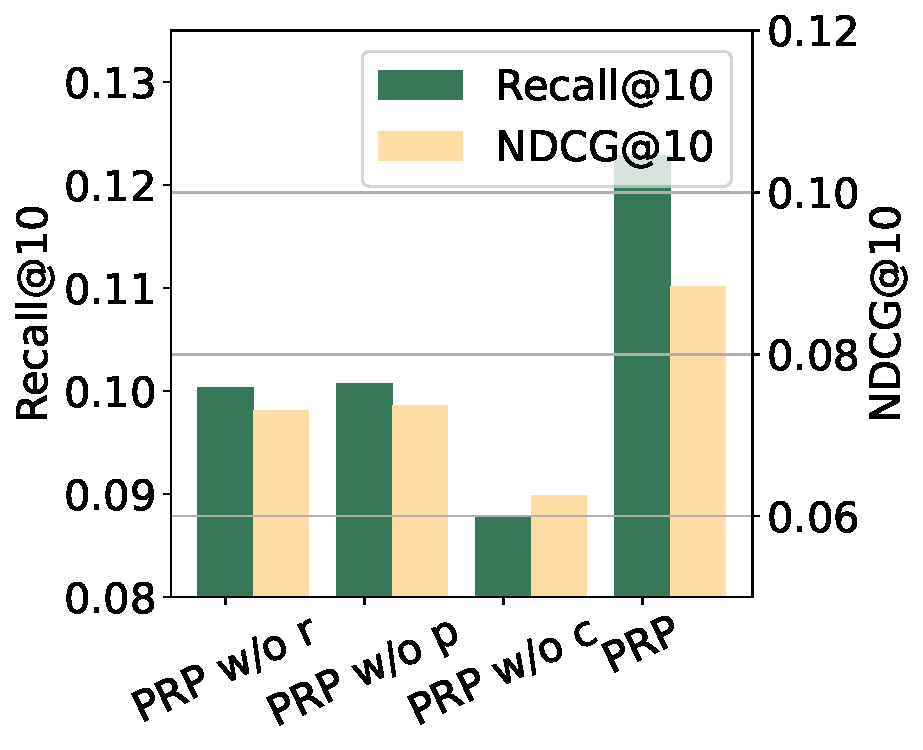
\includegraphics[width=\linewidth]{fig/ablation_Gowalla.pdf}
\label{fig:ablation_Gowalla}
\end{minipage}
}
\subfigure[Yelp]{
\begin{minipage}[t]{0.207\linewidth}
\centering
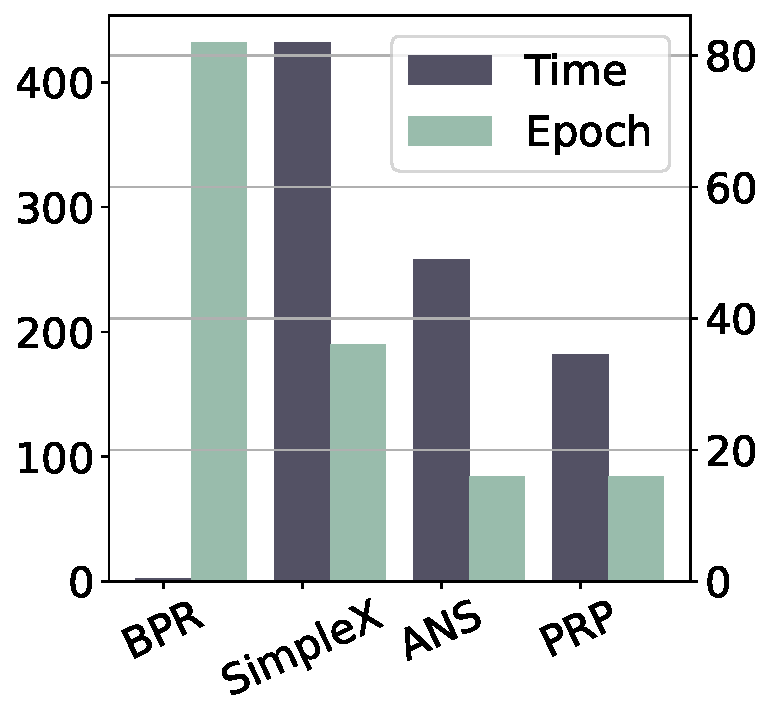
\includegraphics[width=\linewidth]{fig/time_Yelp.pdf}
\label{fig:time_Yelp}
\end{minipage}
}
\subfigure[Gowalla]{
\begin{minipage}[t]{0.207\linewidth}
\centering
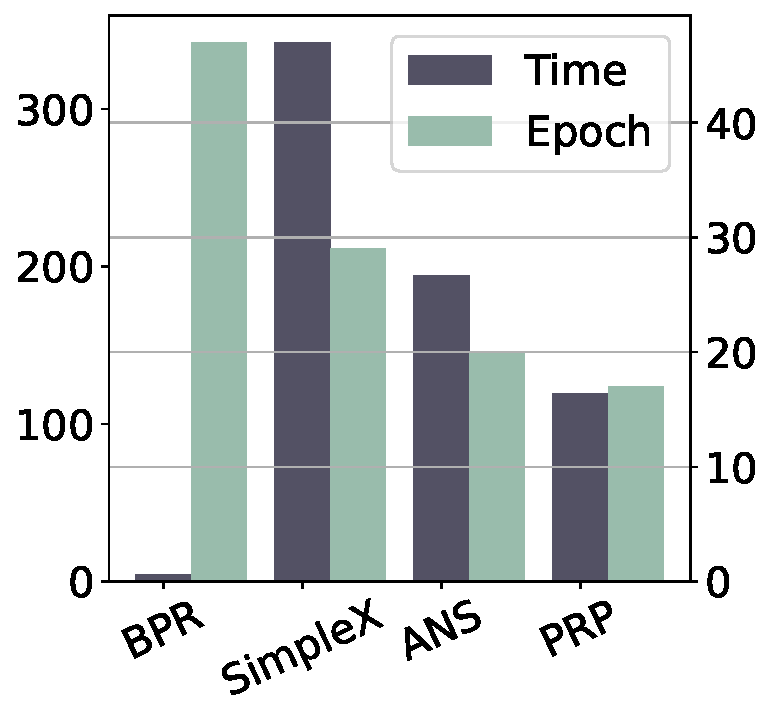
\includegraphics[width=\linewidth]{fig/time_Gowalla.pdf}
\label{fig:time_Gowalla}
\end{minipage}
}
\caption{Experimental results to demonstrate the ablation study and efficiency analysis.}
\label{fig:trap}
\end{figure*}

\textbf{Ablation Study}. We analyze the effectiveness of different components through the following variants: (1) PRP without ranker (PNN w/o r), (2) PRP without $\mathcal{L}_p$ (PNN w/o p), (3) PRP without confidence (PNN w/o c). The results, presented in Figure~\ref{fig:ablation_foursquare}, ~\ref{fig:ablation_Gowalla} indicate that each component positively contributes to model performance. In essence, these three components ensure that the model effectively utilizes accurate ranking information, underscoring the importance of constructing a reasonable ranking. If the ranking is incorrect, the ranking loss becomes meaningless.

\textbf{Efficiency Analysis}. Consistent with previous works~\cite{MZW21, WYM22, ZCL23}, we compare the efficiency of PRP with other representative methods (BPR, SimpleX, and ANS). Figure~\ref{fig:time_Yelp},~\ref{fig:time_Gowalla} present the average training time (sec.) per epoch and the number of epochs required to converge. As anticipated, BPR is the most efficient due to its simplicity. SimpleX, on the other hand, shows the least efficiency, attributed to its dependence on massive negative samples and filtering of uninformative ones. PRP emerges as the second most efficient method. Given its outstanding performance, we assert that PRP stands out as a highly desirable choice.
